\section{Artificial Neural Networks}
          
Artificial Neural Networks are a machine learning model inspired by the human brain. The basic idea behind artificial neural networks is to model the electrochemical activity of single brain cells, called neurons. Figure \ref{fig:neuron} shows the mathematical model of single artificial neuron.
\\
\tikzstyle{inputNode}=[draw,circle,minimum size=10pt,inner sep=0pt]
\tikzstyle{stateTransition}=[->, thick]
\begin{figure}[h]
\centering
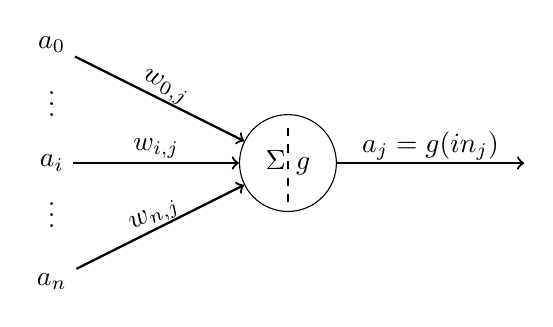
\begin{tikzpicture}
	\node[draw,circle,minimum size=35pt,inner sep=0pt] (x) at (0,0) {$\mathlarger{\mathlarger{\Sigma \textbf{   } g}}$};

	\node (x0) at (-3, 1.5)  {$\tiny a_0$};
	\node (xi)  at (-3, 0)     {$\tiny a_i$};
	\node (xn) at (-3, -1.5) {$\tiny a_n$};

	\draw[stateTransition] (x0) to node [above=-3, sloped, sloped, midway] {$w_{0, j}$} (x);
	\draw[stateTransition] (xi)  to node [above=-2] {$w_{i,j}$} (x);
	\draw[stateTransition] (xn) to node [above=-3, sloped, midway] {$w_{n, j}$} (x);
	
	\node (dots) at (-3,  0.85) {$\vdots$};
	\node (dots) at (-3, -0.55) {$\vdots$};
	
	\draw[stateTransition] (x) -- (3,0) node [midway,above=-0.1cm] {$ \mathsmaller{a_j = g(in_j)}$};

	\draw[dashed] (0,-0.50) -- (0,0.50);
\end{tikzpicture}
\caption{Schematic description of an artificial neuron}
\label{fig:neuron}
\end{figure}

A neural network is composed of several neurons. These neurons are connected by directed links, called synapis. The synapsis propagate the activation from neuron $i$ to neuron $j$. It has an associated weight called $w_{i,j}$, which denotes the strength of the synapsis. 
\\
\\
It is common to add an additonal neuron to the input neurons of each neuron. This neuron is called the bias neuron and has a constant activation, allowing to shift the neurons output by a certain value. This is often important for successfull learning. The bias neuron of neuron $j$ is denoted by $bias_j$
\\
\\
A neurons weighted input is calculated the following way:

\begin{equation*}
in_j = bias_j + \sum\limits_{i \in Input_j} w_{i,j} a_i.
\end{equation*}

To calculate the activation of the neuron, the activation function $g$ is applied to the weighted input and the bias neuron:

\begin{equation*}
a_j = g(in_j).
\end{equation*}
\\
Typical activation functions are the hyperbolic tangent or sigmoid function. An important property of the activation function is to provide a smooth transition as the input value changes. Furthermore it has to be derivable, to allow application of the backpropagation algortihm, I will introduce later. 


\subsection{Structure} 

There are two fundamentally distinct ways to connect the neurons in a neural network. On the one hand there are feedforward networks, on the other hand there are recurrent networks.
\\
\\
In feedforward networks all connections are directed in the same direction. This makes the network an acyclic graph and the activations following a certain direction. Due to the fact, that a neurons input is only affected by the preceeding neurons and the neurons output only affects the succeeding neurons, there are no loops. Thus the neuronal network has no internal state and represents a function of the input. 
\\
\\
Recurrent networks allow for such loops. Thus the output of certain neurons can be used as input to these neurons again. This makes the networks behavior far more complex to understand, but also allows the neuronal network to preserve an internal state. That allows the neuron to have some kind of short term memory.
\\
\\
In this article I will focus on feedforward neuronal networks. It is common to arrange the neurons of feedforward networks in so called layers. These layers are used to bundle a set of neurons. The layers are ordered in the neural network and each layer uses the preceeding layer as input. The first layer is called the input layer and the last layer is called the output layer. The layers between the input and output layers are called hidden layers. Neural networks without hidden layers are called perceptron networks and neural networks with multiple hidden layers are called multilayer networks. 
\\
\begin{figure}[h]
	\centering

	\tikzstyle{neuron}=[draw, circle, minimum size=19pt, inner sep=0pt]

	\begin{subfigure}{.3333\textwidth}
		\centering
		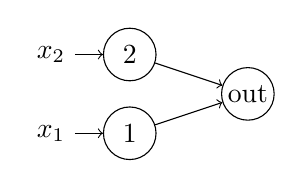
\begin{tikzpicture}
			\node[neuron] (n1) at (0,0)    {1};
			\node[neuron] (n2) at (0,1)    {2};
			\node[neuron] (nout) at (1.5,0.5) {out};
			
			\draw [->] (n1) -- (nout);
			\draw [->] (n2) -- (nout);
			
			\node (x1) at (-1, 0) {$x_1$};
			\node (x2) at (-1, 1) {$x_2$};
			\draw [->] (x1) -- (n1);
			\draw [->] (x2) -- (n2);
			
		\end{tikzpicture}
    	 \caption{}
    \end{subfigure}%    
    % 
    \begin{subfigure}{.3333\textwidth}
		\centering
		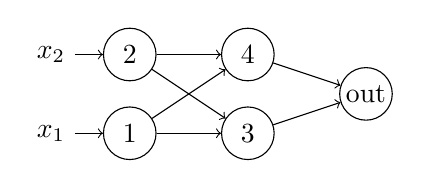
\begin{tikzpicture}
			\node[neuron] (n1) at (0,0)    {1};
			\node[neuron] (n2) at (0,1)    {2};
			\node[neuron] (n3) at (1.5,0)    {3};
			\node[neuron] (n4) at (1.5,1)    {4};
			\node[neuron] (nout) at (3,0.5) {out};
			
			\draw [->] (n1) -- (n3);
			\draw [->] (n1) -- (n4);
			\draw [->] (n2) -- (n3);
			\draw [->] (n2) -- (n4);
			\draw [->] (n3) -- (nout);
			\draw [->] (n4) -- (nout);
			
			\node (x1) at (-1, 0) {$x_1$};
			\node (x2) at (-1, 1) {$x_2$};
			\draw [->] (x1) -- (n1);
			\draw [->] (x2) -- (n2);
			
		\end{tikzpicture}
        \caption{}
	\end{subfigure}%
	
	\caption{Shown are two network architectures for approximating the XOR-function. (a) Shows a perceptron network. (b) Shows a feedforward network with an hidden layer of two neurons}
	\label{fig:xor}
\end{figure}

The networks shown in Figure \ref{fig:xor} can be trained to compute the XOR-function. In Table \ref{tab:xor} you can see the truth table of the XOR-function and the outputs of the two displayed networks.
\\
\begin{table}[h]
  \centering
  \begin{tabular}[c]{cccrr}
    \hline
    \multicolumn{3}{l}{XOR data} 		& \multicolumn{2}{l}{network output}	\\
    \hline
    $x_1$ 		& $x_2$		& $y$	 		& 	perceptron 	& 	multilayer 	\\
    \hline
    0 				& 0 				& 0				& .50				& .00				\\
    0 				& 1 				& 1				& .50 				& .99 				\\
    1 				& 0 				& 1				& .50 				& .99 				\\
    1 				& 1 				& 0				& .50 				& .00 				\\
    \hline
  \end{tabular}
  \caption{output of different networks on XOR data after 50000 training epochs}
  \label{tab:xor}
  
\end{table}

As you can see, the perceptron network is not able to compute the XOR-function. The multilayer network on the other hand can compute the XOR-function easily. The reason for that result is, that an perceptron can only compute linearly seperable functions. To compute more complex functions more layers are required. Actually, it can be shown, that a feedforward neural network with one sufficiently large hidden layer can compute any continuous function of the inputs with arbitrary accuracy.  An feedforward network with two layers can compute even discountinuous functions. 


\subsection{Learning}

The natural question arises, how to train a feedforward neural network. In the following I will introduce the backpropagation algorithm, which can be used to train such a network. 
\\
\\
Interpreting the feedforward neural network as a vector function helps understanding the backpropagation algorithm. Each neuron is interpreted as component of the vector, representing its layer. To calculate the output of such a neural network, the activations of each layers neurons are computed consecutively, as shown in the following algorithm: 
\\
\\
\begin{algorithm}[H]
	\KwData{ input vector $x$ }
	\KwResult{ activations $a_i$ for all neurons }
	\For{ neuron $j$ in input layer } {
		$a_j \leftarrow x_j $
	}
	\For{ $l=2$ to layer count } {
		\For {neuron $j$ of neurons in $l$ } {
			$a_j \leftarrow g(\sum\limits_{i \in Input_j} w_{i,j} a_i + bias_j)$
		}
	}
	\For{ neuron $k$ in output layer }  {
		$h_k \leftarrow a_k$	
	}
\end{algorithm}
~\\
After the output vector $h$ of the network is calculated for a certain input, the networks output and the target output $y$ can be compared. The output error is calculated using an error function. After the output error is calculated, it is neccessary to compute the error of the neurons in the previous layers. This is done by backpropagating the error. 
\\
\\
It is common to use squared error as error function, which is shown in the following:

\begin{equation*}
L_2 = (y_k - h_k)^2.
\end{equation*}
\\
To reduce the error $L_2$ of the networks output, we can change $h_k$. To change $h_k$, we can thus change $in_k$, because $h_k = g(in_k)$. The amount about which to change $in_k$ can be obtained by deriving $L_2$ with respect to $in_k$: 

\begin{equation*}
\frac{ \delta L_2 }{ \delta in_k }    =    \frac{ \delta ((y_k - h_k)^2) }{ \delta in_k }     =      \frac{ \delta (y_k - g(in_k)) }{ \delta in_k }  *  2 * (y_k - g(in_k) )   =   g'(in_k) * 2 * (y_k - g(in_k)).
\end{equation*}
\\
By leaving out the $2$ as constant factor and defining $Err_k = y_k - g(in_k)$ , we define a modified error:

\begin{equation}
\label{eq:bp:errout}
\Delta_k = Err_k * g'(in_k).
\end{equation}
\\
This error will later be used, to compute the weight update of the network. If the network contains hidden layers, it is neccessary to compute a similar measure of error for the hidden layer neurons too. To do this, we can backpropagate the error to these neurons. Neuron $j$ affects the error $\Delta_k$ of each neuron $k$ it connects to as input neuron by a certain amount, scaled by the weight $w_{j,k}$ from $j$ to $k$. The idea is to add up the error $j$ produces: 

\begin{equation}
\label{eq:bp:errhid}
\Delta j = g'(in_j) * \sum\limits_k w_{j,k} * \Delta_k.
\end{equation}

As the error $\Delta_j$ for every neuron in the network is computed, the error can be used to update the weights of every synapsis. The weight update is aimed to reduce the general error $L_2$. To update the weights, the following rule is used:

\begin{equation}
\label{eq:bp:wupd}
w_{i,j} \leftarrow w_{i,j} + \alpha * a_i * \Delta_j.
\end{equation}

Here $\alpha$ is the learning rate, determining how much to change the weights each weight update. To understand the weight update rule, it is important to know, that $\frac{ \delta L_2 }{ \delta w_{i,j} } = -a_i * \Delta_j$, both for the output and hidden layers. Because of this, to reduce the output error by changing $w_{i,j}$, the weight $w_{i,j}$ has to be changed by $\frac{ \delta L_2 }{ \delta w_{i,j} }$. Thus the weight update rule changes each weight in a way, so that the error is reduced. 
\\
\\
To update the biases, similar considerations are applied. Due to $\frac{ \delta L_2 }{ \delta bias_i } = \Delta_j$, the bias update rule becomes: 

\begin{equation}
\label{eq:bp:bupd}
bias_i \leftarrow \alpha * \Delta_i.
\end{equation}

The final algorithm follows the following steps for each training example: 
\begin{itemize}
\item Do feedforward pass	
\item Calculate output errors using Equation \ref{eq:bp:errout}
\item Backpropagate errors using Equation \ref{eq:bp:errhid}
\item Do weight update using Equation \ref{eq:bp:wupd} and bias update using Equation \ref{eq:bp:bupd}
\end{itemize}
~\\ 
The actual algorithm becomes:
\\
\\
\begin{algorithm}[H]
	\KwData{ set of examples, each containing input $x$ and target $y$ }
	\KwResult{ activations $a_i$ for all neurons }
	
	do forward step, calculating $in_j$, $a_j$ for each neuron $j$\\
	\For{ neuron $k$ in output layer } {
		$\Delta_k \leftarrow (y_k - a_k) * g'(in_k)$
	}
	\For{ $l=2$ to $L$ } {
		\For {neuron $i$ of neurons in $l$ } {
			$ \Delta_i \leftarrow g'(in_i) * \sum_j w_{i,j} * \Delta_j$
		}
	}
	\For{ weight $w_{i,j}$ of each synapsis in network } {
		$ w{i,j} \leftarrow w_{i,j} + \alpha * a_i * \Delta_j $
	}
	\For { neuron $i$ in network } {
		$ bias_i \leftarrow  \alpha * \Delta_i $
	}
\end{algorithm}
~\\
 
 
\subsection{Practical usage of Neural Networks}

% ANN on iris versicolor dataset 
% Describe problem: 3 classes, measured data, data source, 150 entries
% Describe class encoding
% Describe nn 4,8,3 sigmoid
% Describe K-Folding 3
% Describe result, accuracy def

To describe the practical usage of neural networks, I apply a feedforward neural network to the Iris data set. The Iris data set is a well studied data set in the area of machine learning. It can be obtained from the UCI Machine Learning Repository \cite{UCI}. The dataset contains 150 entries, each denoting several attributes of an Iris plant and its classification. The attributes are sepal length in cm, sepal width in cm, petal length in cm and petal width in cm. The possible classifications are Iris Setosa, Iris Versicolour and Iris Virginica. My goal is to train a neural network to classify each entry by using the attributes as input. 
\\
\\
The classes are encoded using one-hot encoding. For this classification problem this leads to the following encoding shown in Table \ref{tab:iris_encoding}.

\begin{table}[tb]
  \centering
  \begin{tabular}[c]{lc}
    \hline
    classification			& $y$ 					\\
    \hline
    Iris Setosa 				& $(1, 0, 0)$		\\
    Iris Versicolour 		& $(0, 1, 0)$		\\
    Iris Virginica 			& $(0, 0, 1)$		\\
    \hline
  \end{tabular}
  \caption{one-hot encoding of Iris dataset}
  \label{tab:iris_encoding}
\end{table}


As model, I use a feedforward neural network with 4 input neurons, one hidden layer of 8 neurons and an output layer of 3 neurons. As activation function I use the $sigmoid$ function. 
\\
\\
To evaluate the network, k-fold cross validation with $k=5$ is used. In addition to the output error I also calculate the accuracy of the network. The accuracy determines, how much of the entries from the test set are classified correct. An entry is considered correctly classified, if for every output neuron $k$: 

\begin{equation*}
y_k =\lfloor h_k \rceil.
\end{equation*}
\\
The accuracy is defined as the percentage of correctly classified entries:

\begin{equation*}
accuracy = \frac{ num_{correct} }{ num_{test} }.
\end{equation*}
\\
The results of my implementation are shown in the below table: 
\\
\\
\begin{table}[h]
  \centering
  \begin{tabular}[c]{crr}
    \hline
    round			& error						& accuracy (\%) 		\\
    \hline
    1					& 0.030					& 100.00					\\
    2					& 0.049					& 96.67					\\
    3					& 0.057					& 93.33					\\
    4					& 0.029					& 100.00					\\
    5					& 0.037					& 100.00					\\
    \hline
    average		& 0.040					& 98.00					\\
    \hline
  \end{tabular}
  \caption{Evaluation results classifier to Iris dataset}
  \label{tab:kfold}
\end{table}
\\
As you can see, my implementation archieved an average accuracy of $98\%$, which is quite typical for this data set. In the table I show a sample output of the trained neural network:
\\
\\
\begin{table}[h]
  \centering
  \begin{tabular}[c]{cccr}
    \hline
    $x$								& output			& target			& error		\\
    \hline
    $(5.5, 2.4, 3.7, 1.0)$ 	& $(0, 1, 0)$ 	& $(0, 1, 0)$  	& $0.00$	\\
    $(5.0, 3.4, 1.5, 0.2)$ 	& $(0, 0, 1)$	& $(0, 0, 1)$   & $0.00$	\\
    $(6.0, 2.9, 4.5, 1.5)$ 	& $(0, 1, 0)$	& $(0, 1, 0)$   & $0.00$	\\
    $(6.0, 2.7, 5.1, 1.6)$ 	& $(1, 0, 0)$ 	& $(0, 1, 0)$ 	& $0.67$	\\
    $(5.8, 2.7, 5.1, 1.9)$ 	& $(1, 0, 0)$ 	& $(1, 0, 0)$   & $0.00$	\\
    \hline
  \end{tabular}
  \caption{Sample output on Iris dataset}
  \label{tab:iris_example}
\end{table}

